% Options for packages loaded elsewhere
\PassOptionsToPackage{unicode}{hyperref}
\PassOptionsToPackage{hyphens}{url}
%
\documentclass[
  10pt,
  ignorenonframetext,
]{beamer}
\usepackage{pgfpages}
\setbeamertemplate{caption}[numbered]
\setbeamertemplate{caption label separator}{: }
\setbeamercolor{caption name}{fg=normal text.fg}
\beamertemplatenavigationsymbolsempty
% Prevent slide breaks in the middle of a paragraph
\widowpenalties 1 10000
\raggedbottom
\setbeamertemplate{part page}{
  \centering
  \begin{beamercolorbox}[sep=16pt,center]{part title}
    \usebeamerfont{part title}\insertpart\par
  \end{beamercolorbox}
}
\setbeamertemplate{section page}{
  \centering
  \begin{beamercolorbox}[sep=12pt,center]{part title}
    \usebeamerfont{section title}\insertsection\par
  \end{beamercolorbox}
}
\setbeamertemplate{subsection page}{
  \centering
  \begin{beamercolorbox}[sep=8pt,center]{part title}
    \usebeamerfont{subsection title}\insertsubsection\par
  \end{beamercolorbox}
}
\AtBeginPart{
  \frame{\partpage}
}
\AtBeginSection{
  \ifbibliography
  \else
    \frame{\sectionpage}
  \fi
}
\AtBeginSubsection{
  \frame{\subsectionpage}
}
\usepackage{lmodern}
\usepackage{amssymb,amsmath}
\usepackage{ifxetex,ifluatex}
\ifnum 0\ifxetex 1\fi\ifluatex 1\fi=0 % if pdftex
  \usepackage[T1]{fontenc}
  \usepackage[utf8]{inputenc}
  \usepackage{textcomp} % provide euro and other symbols
\else % if luatex or xetex
  \usepackage{unicode-math}
  \defaultfontfeatures{Scale=MatchLowercase}
  \defaultfontfeatures[\rmfamily]{Ligatures=TeX,Scale=1}
\fi
\usetheme[]{Warsaw}
\usecolortheme{whale}
\usefonttheme{structuresmallcapsserif}
% Use upquote if available, for straight quotes in verbatim environments
\IfFileExists{upquote.sty}{\usepackage{upquote}}{}
\IfFileExists{microtype.sty}{% use microtype if available
  \usepackage[]{microtype}
  \UseMicrotypeSet[protrusion]{basicmath} % disable protrusion for tt fonts
}{}
\makeatletter
\@ifundefined{KOMAClassName}{% if non-KOMA class
  \IfFileExists{parskip.sty}{%
    \usepackage{parskip}
  }{% else
    \setlength{\parindent}{0pt}
    \setlength{\parskip}{6pt plus 2pt minus 1pt}}
}{% if KOMA class
  \KOMAoptions{parskip=half}}
\makeatother
\usepackage{xcolor}
\IfFileExists{xurl.sty}{\usepackage{xurl}}{} % add URL line breaks if available
\IfFileExists{bookmark.sty}{\usepackage{bookmark}}{\usepackage{hyperref}}
\hypersetup{
  pdftitle={Import Data},
  pdfauthor={Jan-Philipp Kolb},
  hidelinks,
  pdfcreator={LaTeX via pandoc}}
\urlstyle{same} % disable monospaced font for URLs
\newif\ifbibliography
\usepackage{color}
\usepackage{fancyvrb}
\newcommand{\VerbBar}{|}
\newcommand{\VERB}{\Verb[commandchars=\\\{\}]}
\DefineVerbatimEnvironment{Highlighting}{Verbatim}{commandchars=\\\{\}}
% Add ',fontsize=\small' for more characters per line
\usepackage{framed}
\definecolor{shadecolor}{RGB}{48,48,48}
\newenvironment{Shaded}{\begin{snugshade}}{\end{snugshade}}
\newcommand{\AlertTok}[1]{\textcolor[rgb]{1.00,0.81,0.69}{#1}}
\newcommand{\AnnotationTok}[1]{\textcolor[rgb]{0.50,0.62,0.50}{\textbf{#1}}}
\newcommand{\AttributeTok}[1]{\textcolor[rgb]{0.80,0.80,0.80}{#1}}
\newcommand{\BaseNTok}[1]{\textcolor[rgb]{0.86,0.64,0.64}{#1}}
\newcommand{\BuiltInTok}[1]{\textcolor[rgb]{0.80,0.80,0.80}{#1}}
\newcommand{\CharTok}[1]{\textcolor[rgb]{0.86,0.64,0.64}{#1}}
\newcommand{\CommentTok}[1]{\textcolor[rgb]{0.50,0.62,0.50}{#1}}
\newcommand{\CommentVarTok}[1]{\textcolor[rgb]{0.50,0.62,0.50}{\textbf{#1}}}
\newcommand{\ConstantTok}[1]{\textcolor[rgb]{0.86,0.64,0.64}{\textbf{#1}}}
\newcommand{\ControlFlowTok}[1]{\textcolor[rgb]{0.94,0.87,0.69}{#1}}
\newcommand{\DataTypeTok}[1]{\textcolor[rgb]{0.87,0.87,0.75}{#1}}
\newcommand{\DecValTok}[1]{\textcolor[rgb]{0.86,0.86,0.80}{#1}}
\newcommand{\DocumentationTok}[1]{\textcolor[rgb]{0.50,0.62,0.50}{#1}}
\newcommand{\ErrorTok}[1]{\textcolor[rgb]{0.76,0.75,0.62}{#1}}
\newcommand{\ExtensionTok}[1]{\textcolor[rgb]{0.80,0.80,0.80}{#1}}
\newcommand{\FloatTok}[1]{\textcolor[rgb]{0.75,0.75,0.82}{#1}}
\newcommand{\FunctionTok}[1]{\textcolor[rgb]{0.94,0.94,0.56}{#1}}
\newcommand{\ImportTok}[1]{\textcolor[rgb]{0.80,0.80,0.80}{#1}}
\newcommand{\InformationTok}[1]{\textcolor[rgb]{0.50,0.62,0.50}{\textbf{#1}}}
\newcommand{\KeywordTok}[1]{\textcolor[rgb]{0.94,0.87,0.69}{#1}}
\newcommand{\NormalTok}[1]{\textcolor[rgb]{0.80,0.80,0.80}{#1}}
\newcommand{\OperatorTok}[1]{\textcolor[rgb]{0.94,0.94,0.82}{#1}}
\newcommand{\OtherTok}[1]{\textcolor[rgb]{0.94,0.94,0.56}{#1}}
\newcommand{\PreprocessorTok}[1]{\textcolor[rgb]{1.00,0.81,0.69}{\textbf{#1}}}
\newcommand{\RegionMarkerTok}[1]{\textcolor[rgb]{0.80,0.80,0.80}{#1}}
\newcommand{\SpecialCharTok}[1]{\textcolor[rgb]{0.86,0.64,0.64}{#1}}
\newcommand{\SpecialStringTok}[1]{\textcolor[rgb]{0.80,0.58,0.58}{#1}}
\newcommand{\StringTok}[1]{\textcolor[rgb]{0.80,0.58,0.58}{#1}}
\newcommand{\VariableTok}[1]{\textcolor[rgb]{0.80,0.80,0.80}{#1}}
\newcommand{\VerbatimStringTok}[1]{\textcolor[rgb]{0.80,0.58,0.58}{#1}}
\newcommand{\WarningTok}[1]{\textcolor[rgb]{0.50,0.62,0.50}{\textbf{#1}}}
\usepackage{longtable,booktabs}
\usepackage{caption}
% Make caption package work with longtable
\makeatletter
\def\fnum@table{\tablename~\thetable}
\makeatother
\usepackage{graphicx,grffile}
\makeatletter
\def\maxwidth{\ifdim\Gin@nat@width>\linewidth\linewidth\else\Gin@nat@width\fi}
\def\maxheight{\ifdim\Gin@nat@height>\textheight\textheight\else\Gin@nat@height\fi}
\makeatother
% Scale images if necessary, so that they will not overflow the page
% margins by default, and it is still possible to overwrite the defaults
% using explicit options in \includegraphics[width, height, ...]{}
\setkeys{Gin}{width=\maxwidth,height=\maxheight,keepaspectratio}
% Set default figure placement to htbp
\makeatletter
\def\fps@figure{htbp}
\makeatother
\setlength{\emergencystretch}{3em} % prevent overfull lines
\providecommand{\tightlist}{%
  \setlength{\itemsep}{0pt}\setlength{\parskip}{0pt}}
\setcounter{secnumdepth}{-\maxdimen} % remove section numbering

\title{Import Data}
\author{Jan-Philipp Kolb}
\date{03 März, 2020}

\begin{document}
\frame{\titlepage}

\begin{frame}{\href{http://uc-r.github.io/data_wrangling/week-3}{FIRST
THINGS TO DO}}
\protect\hypertarget{first-things-to-do}{}

Don't try to kiss your data on the first date; rather, you just want to
get to know the data:

\begin{enumerate}
\tightlist
\item
  \textbf{Import the data}
\item
  Review the codebook
\item
  Learn about the data
\item
  Quick visual understanding of the data
\end{enumerate}

\end{frame}

\begin{frame}{Data import}
\protect\hypertarget{data-import}{}

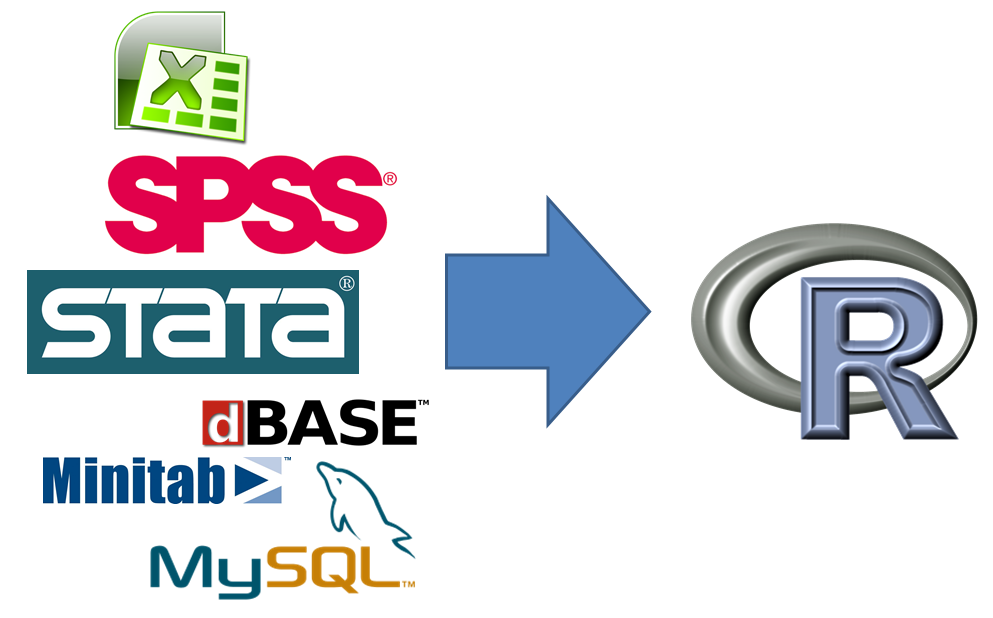
\includegraphics{figure/Datenimport.PNG}

\end{frame}

\begin{frame}{Import data with Rstudio}
\protect\hypertarget{import-data-with-rstudio}{}

\begin{block}{Rstudio functionality to import data}

\begin{itemize}
\tightlist
\item
  Environment - Import Dataset - choose file type
\end{itemize}

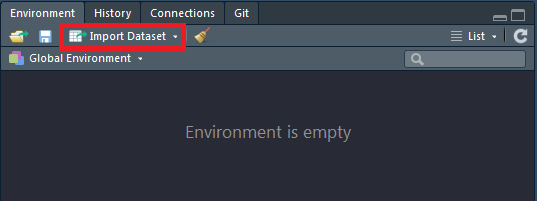
\includegraphics{figure/rstudio_import.PNG}

\end{block}

\end{frame}

\begin{frame}{Where to find data}
\protect\hypertarget{where-to-find-data}{}

\begin{block}{Browse Button in RStudio}

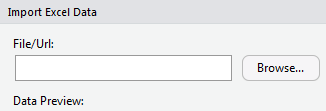
\includegraphics{figure/importBrowse.PNG}

\end{block}

\begin{block}{Code preview in Rstudio}

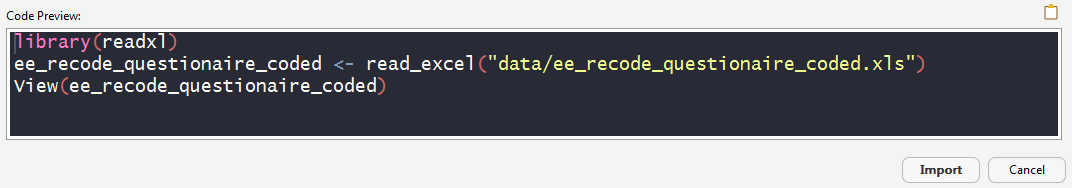
\includegraphics{figure/codepreview.PNG}

\end{block}

\end{frame}

\begin{frame}{\href{http://www.sthda.com/english/wiki/importing-data-into-r}{Import
\texttt{.csv} data}}
\protect\hypertarget{import-.csv-data}{}

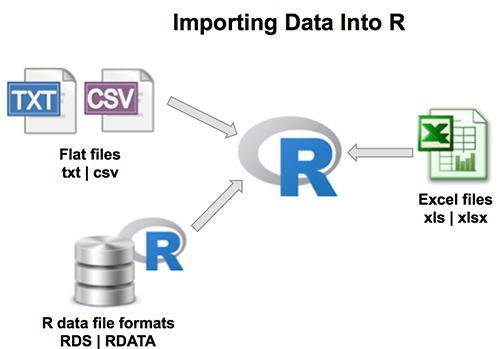
\includegraphics{figure/importing-data-into-r.png}

\end{frame}

\begin{frame}[fragile]{Import of csv data}
\protect\hypertarget{import-of-csv-data}{}

\begin{itemize}
\tightlist
\item
  \texttt{read.csv} is a command available in base package
\item
  Excel data can be saved as \texttt{.csv} in Excel
\item
  Then \texttt{read.csv()} can be used to read in the data.
\item
  For German data, you may need \texttt{read.csv2()} because of the
  comma separation.
\end{itemize}

\begin{Shaded}
\begin{Highlighting}[]
\NormalTok{dat <-}\StringTok{ }\KeywordTok{read.csv}\NormalTok{(}\StringTok{"../data/ZA5666_v1-0-0.csv"}\NormalTok{)}
\end{Highlighting}
\end{Shaded}

If it's German data:

\begin{Shaded}
\begin{Highlighting}[]
\NormalTok{datd <-}\StringTok{ }\KeywordTok{read.csv2}\NormalTok{(}\StringTok{"../data/ZA5666_v1-0-0.csv"}\NormalTok{)}
\end{Highlighting}
\end{Shaded}

\begin{Shaded}
\begin{Highlighting}[]
\NormalTok{dat <-}\StringTok{ }\KeywordTok{read.csv}\NormalTok{(}\StringTok{"../data/datahub_refugee.csv"}\NormalTok{)}
\end{Highlighting}
\end{Shaded}

\end{frame}

\begin{frame}[fragile]{The result - a \texttt{data.frame}}
\protect\hypertarget{the-result---a-data.frame}{}

\begin{itemize}
\tightlist
\item
  the following \texttt{data.frame} is a small excerpt from the data:
\end{itemize}

\begin{Shaded}
\begin{Highlighting}[]
\KeywordTok{head}\NormalTok{(dat)}
\end{Highlighting}
\end{Shaded}

\begin{verbatim}
##   Country.Name Country.Code Year   Value
## 1   Arab World          ARB 1990 4235545
## 2   Arab World          ARB 1991 3811595
## 3   Arab World          ARB 1992 4000509
## 4   Arab World          ARB 1993 4189545
## 5   Arab World          ARB 1994 4352945
## 6   Arab World          ARB 1995 4337009
\end{verbatim}

\end{frame}

\begin{frame}[fragile]{The package \texttt{readxl}}
\protect\hypertarget{the-package-readxl}{}

\begin{Shaded}
\begin{Highlighting}[]
\KeywordTok{install.packages}\NormalTok{(}\StringTok{"readxl"}\NormalTok{)}
\end{Highlighting}
\end{Shaded}

\begin{itemize}
\tightlist
\item
  \href{https://stackoverflow.com/questions/7049272/importing-excel-files-into-r-xlsx-or-xls}{\textbf{\texttt{readxl}
  has no external dependencies}}
\item
  \texttt{readxl} supports both the legacy \texttt{.xls} format and the
  modern xml-based \texttt{.xlsx} format.
\end{itemize}

\begin{Shaded}
\begin{Highlighting}[]
\KeywordTok{library}\NormalTok{(readxl)}
\NormalTok{ab <-}\StringTok{ }\KeywordTok{read_excel}\NormalTok{(}\StringTok{"../data/datahub_names_sa.xlsx"}\NormalTok{)}
\KeywordTok{head}\NormalTok{(ab)}
\end{Highlighting}
\end{Shaded}

\begin{verbatim}
## # A tibble: 6 x 3
##   ...1  X1           X2      
##   <chr> <chr>        <chr>   
## 1 1     0.0036749995 JOHN    
## 2 2     0.0036418888 JOHANNES
## 3 3     0.0031182974 DAVID   
## 4 4     0.0030492798 MICHAEL 
## 5 5     0.0029608373 JACOBUS 
## 6 6     0.0027139047 MARIA
\end{verbatim}

\end{frame}

\begin{frame}[fragile]{Import SPSS files}
\protect\hypertarget{import-spss-files}{}

\begin{block}{Import GESIS Panel data}

\begin{itemize}
\tightlist
\item
  library \texttt{haven} - import and export `SPSS', `Stata' and `SAS'
  files
\item
  the result of this import command is a tibble
\end{itemize}

\begin{Shaded}
\begin{Highlighting}[]
\KeywordTok{library}\NormalTok{(haven)}
\NormalTok{dataset <-}\StringTok{ }\KeywordTok{read_sav}\NormalTok{(}\StringTok{"../data/datahub_government_africa.sav"}\NormalTok{)}
\end{Highlighting}
\end{Shaded}

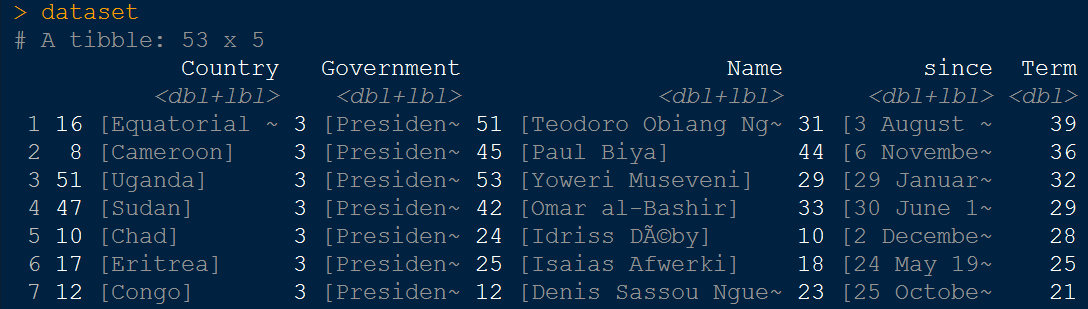
\includegraphics{figure/governmentdata_africa.PNG}

\end{block}

\end{frame}

\begin{frame}[fragile]{Import data from the web}
\protect\hypertarget{import-data-from-the-web}{}

\begin{block}{Austrian microcensus}

Files can also be imported directly from the Internet:

\begin{Shaded}
\begin{Highlighting}[]
\KeywordTok{library}\NormalTok{(foreign)}
\NormalTok{link <-}\StringTok{ "http://www.statistik.at/web_de/static/}
\StringTok{mz_2013_sds_-_datensatz_080469.sav"}

\NormalTok{?read.spss}
\NormalTok{Dat <-}\StringTok{ }\KeywordTok{read.spss}\NormalTok{(link,}\DataTypeTok{to.data.frame=}\NormalTok{T)}
\end{Highlighting}
\end{Shaded}

\end{block}

\end{frame}

\begin{frame}[fragile]{Import \texttt{stata} files}
\protect\hypertarget{import-stata-files}{}

\begin{block}{Import newer \texttt{.dta} files}

\begin{itemize}
\tightlist
\item
  With \texttt{read.dta13} stata files from version 13 (and higher) can
  be imported
\end{itemize}

\begin{Shaded}
\begin{Highlighting}[]
\KeywordTok{library}\NormalTok{(readstata13)}
\NormalTok{dat_stata <-}\StringTok{ }\KeywordTok{read.dta13}\NormalTok{(}\StringTok{"../data/example_gp.dta"}\NormalTok{)}
\end{Highlighting}
\end{Shaded}

\end{block}

\begin{block}{Import \texttt{stata} files - older versions}

\begin{Shaded}
\begin{Highlighting}[]
\KeywordTok{library}\NormalTok{(foreign)}
\NormalTok{dat_stata12 <-}\StringTok{ }\KeywordTok{read.dta}\NormalTok{(}\StringTok{"../data/example_gp_stata12.dta"}\NormalTok{)}
\end{Highlighting}
\end{Shaded}

\end{block}

\end{frame}

\begin{frame}{The library \texttt{readstata13}}
\protect\hypertarget{the-library-readstata13}{}

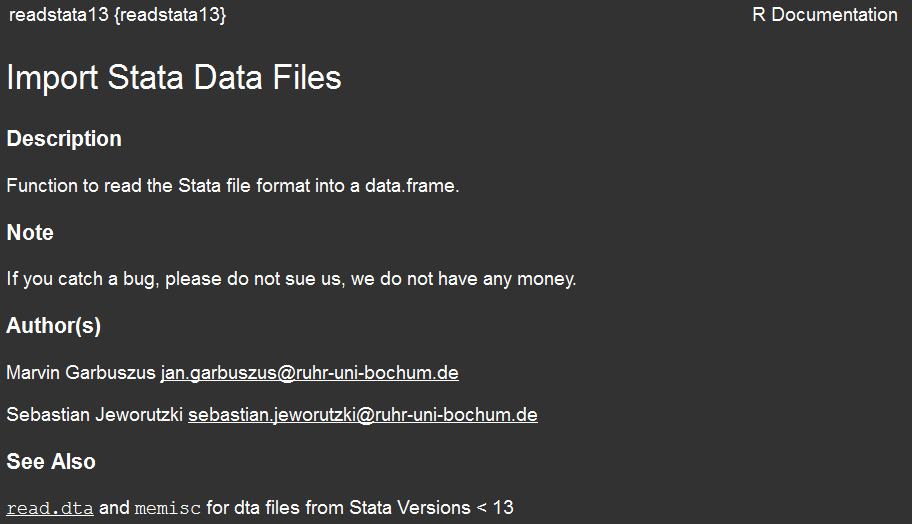
\includegraphics{figure/readstata13.PNG}

\end{frame}

\begin{frame}[fragile]{Import - GESIS Panel data}
\protect\hypertarget{import---gesis-panel-data}{}

\begin{block}{\texttt{convert.factors} argument}

\begin{Shaded}
\begin{Highlighting}[]
\KeywordTok{library}\NormalTok{(readstata13)}
\end{Highlighting}
\end{Shaded}

\begin{Shaded}
\begin{Highlighting}[]
\NormalTok{datf <-}\StringTok{ }\KeywordTok{read.dta13}\NormalTok{(}\StringTok{"../data/example_gp.dta"}\NormalTok{,}
                  \DataTypeTok{convert.factors =}\NormalTok{ F)}
\KeywordTok{head}\NormalTok{(datf}\OperatorTok{$}\NormalTok{bbzc007a)}
\end{Highlighting}
\end{Shaded}

\begin{verbatim}
## NULL
\end{verbatim}

\end{block}

\begin{block}{For comparison - import without this argument}

\begin{Shaded}
\begin{Highlighting}[]
\NormalTok{dat <-}\StringTok{ }\KeywordTok{read.dta13}\NormalTok{(}\StringTok{"../data/example_gp.dta"}\NormalTok{)}
\KeywordTok{head}\NormalTok{(dat}\OperatorTok{$}\NormalTok{bbzc007a)}
\end{Highlighting}
\end{Shaded}

\begin{verbatim}
## NULL
\end{verbatim}

\end{block}

\end{frame}

\begin{frame}[fragile]{The argument \texttt{convert.factors\ =\ F}}
\protect\hypertarget{the-argument-convert.factors-f}{}

\begin{block}{More information on \texttt{.dta} import}

\begin{Shaded}
\begin{Highlighting}[]
\NormalTok{?read.dta13}
\end{Highlighting}
\end{Shaded}

\begin{itemize}
\item
  \texttt{convert.factors} - logical. If \texttt{TRUE}, factors from
  Stata value labels are created.
\item
  It might be useful to import the dataset twice - with and without
  value labels\ldots{}
\item
  \texttt{nonint.factors}- logical. If \texttt{TRUE}, factors labels
  will be assigned to variables of type float and double.
\item
  The import must be controlled, because otherwise errors can easily
  happen.
\end{itemize}

\end{block}

\end{frame}

\begin{frame}[fragile]{Get stata attributes}
\protect\hypertarget{get-stata-attributes}{}

\begin{Shaded}
\begin{Highlighting}[]
\NormalTok{att_dat <-}\StringTok{ }\KeywordTok{attributes}\NormalTok{(dat)}
\KeywordTok{head}\NormalTok{(}\KeywordTok{names}\NormalTok{(att_dat))}
\end{Highlighting}
\end{Shaded}

\begin{verbatim}
## NULL
\end{verbatim}

\begin{block}{Example: the variable names}

\begin{Shaded}
\begin{Highlighting}[]
\KeywordTok{head}\NormalTok{(att_dat}\OperatorTok{$}\NormalTok{names)}
\end{Highlighting}
\end{Shaded}

\begin{verbatim}
## NULL
\end{verbatim}

\end{block}

\end{frame}

\begin{frame}[fragile]{Get an initial overview of the data}
\protect\hypertarget{get-an-initial-overview-of-the-data}{}

\begin{Shaded}
\begin{Highlighting}[]
\KeywordTok{View}\NormalTok{(datf)}
\end{Highlighting}
\end{Shaded}

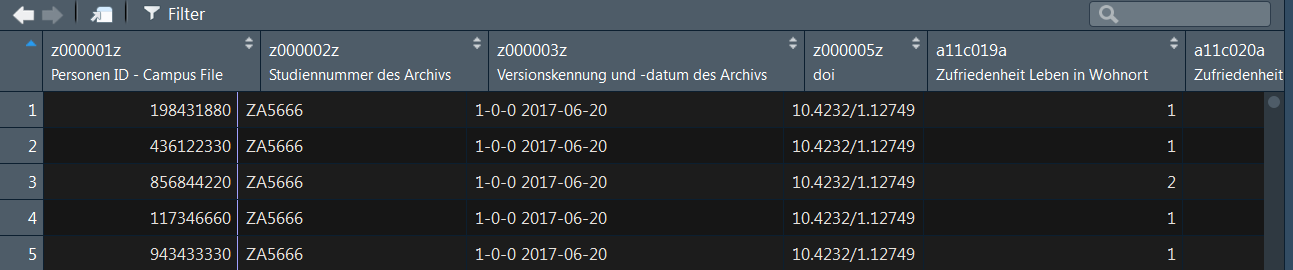
\includegraphics{figure/firstoverview.PNG}

\begin{itemize}
\tightlist
\item
  You can get the same in RStudio if you click on the dataset icon in
  the environment menue
\end{itemize}

\end{frame}

\begin{frame}[fragile]{\href{https://cran.r-project.org/web/packages/rio/vignettes/rio.html}{\textbf{The
library \texttt{rio}}}}
\protect\hypertarget{the-library-rio}{}

\begin{Shaded}
\begin{Highlighting}[]
\KeywordTok{install.packages}\NormalTok{(}\StringTok{"rio"}\NormalTok{)}
\end{Highlighting}
\end{Shaded}

\begin{Shaded}
\begin{Highlighting}[]
\KeywordTok{library}\NormalTok{(}\StringTok{"rio"}\NormalTok{)}
\NormalTok{x <-}\StringTok{ }\KeywordTok{import}\NormalTok{(}\StringTok{"../data/ZA5666_v1-0-0.csv"}\NormalTok{)}
\NormalTok{y <-}\StringTok{ }\KeywordTok{import}\NormalTok{(}\StringTok{"../data/ZA5666_v1-0-0_Stata12.dta"}\NormalTok{)}
\NormalTok{z <-}\StringTok{ }\KeywordTok{import}\NormalTok{(}\StringTok{"../data/ZA5666_v1-0-0_Stata14.dta"}\NormalTok{)}
\end{Highlighting}
\end{Shaded}

\begin{itemize}
\tightlist
\item
  \href{https://cran.r-project.org/web/packages/rio/README.html}{\textbf{rio:
  A Swiss-Army Knife for Data I/O}}
\end{itemize}

\end{frame}

\begin{frame}[fragile]{\href{https://www.statmethods.net/input/importingdata.html}{The
package \texttt{Hmisc}}}
\protect\hypertarget{the-package-hmisc}{}

\begin{quote}
For SPSS and SAS I would recommend the Hmisc package for ease and
functionality.
\end{quote}

\begin{Shaded}
\begin{Highlighting}[]
\KeywordTok{library}\NormalTok{(Hmisc)}
\NormalTok{mydata <-}\StringTok{ }\KeywordTok{spss.get}\NormalTok{(}\StringTok{"c:/mydata.por"}\NormalTok{, }\DataTypeTok{use.value.labels=}\OtherTok{TRUE}\NormalTok{)}
\CommentTok{# last option converts value labels to R factors}
\end{Highlighting}
\end{Shaded}

\begin{block}{Import SAS data}

\begin{Shaded}
\begin{Highlighting}[]
\NormalTok{mydata <-}\StringTok{ }\KeywordTok{sasxport.get}\NormalTok{(}\StringTok{"c:/mydata.xpt"}\NormalTok{)}
\CommentTok{# character variables are converted to R factors}
\end{Highlighting}
\end{Shaded}

\end{block}

\end{frame}

\begin{frame}{The working directory}
\protect\hypertarget{the-working-directory}{}

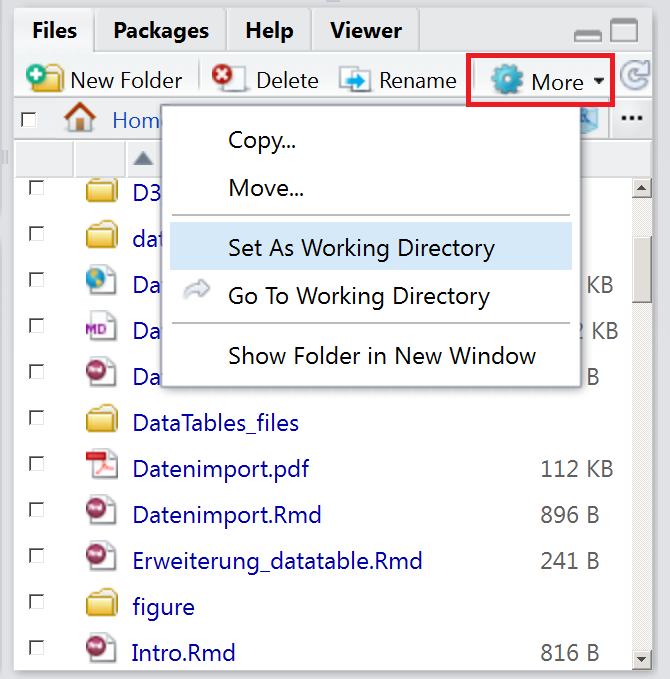
\includegraphics{figure/SetWD.PNG}

\end{frame}

\begin{frame}{\ldots{}}
\protect\hypertarget{section}{}

\begin{itemize}
\tightlist
\item
  If the data is on a different drive in Windows
\end{itemize}

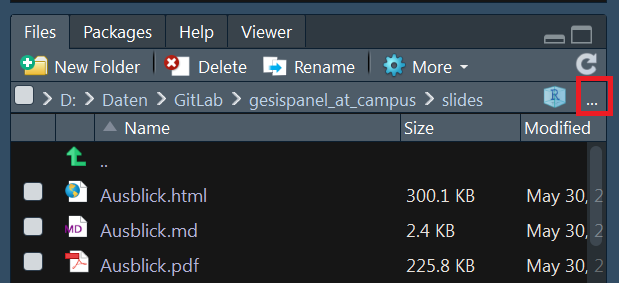
\includegraphics{figure/ptptpt.PNG}

\end{frame}

\begin{frame}[fragile]{The working directory II}
\protect\hypertarget{the-working-directory-ii}{}

This way you can find out which directory you are currently in

\begin{Shaded}
\begin{Highlighting}[]
\KeywordTok{getwd}\NormalTok{()}
\end{Highlighting}
\end{Shaded}

So you can change the working directory:

You create an object in which you save the path:

\begin{Shaded}
\begin{Highlighting}[]
\NormalTok{main.path <-}\StringTok{ "C:/"} \CommentTok{# Example for Windows}
\NormalTok{main.path <-}\StringTok{ "/users/Name/"} \CommentTok{# Example for Mac}
\NormalTok{main.path <-}\StringTok{ "/home/user/"} \CommentTok{# Example for Linux}
\end{Highlighting}
\end{Shaded}

And then change the path with \texttt{setwd()}

\begin{Shaded}
\begin{Highlighting}[]
\KeywordTok{setwd}\NormalTok{(main.path)}
\end{Highlighting}
\end{Shaded}

On Windows it is important to use slashs instead of backslashes.

\end{frame}

\begin{frame}[fragile]{Change working directory}
\protect\hypertarget{change-working-directory}{}

\begin{itemize}
\tightlist
\item
  You can also use the tab key to get the autocompletion.
\end{itemize}

\begin{Shaded}
\begin{Highlighting}[]
\KeywordTok{getwd}\NormalTok{()}
\end{Highlighting}
\end{Shaded}

\begin{verbatim}
## [1] "D:/github/intror2020/slides"
\end{verbatim}

\begin{Shaded}
\begin{Highlighting}[]
\KeywordTok{setwd}\NormalTok{(}\StringTok{".."}\NormalTok{)}
\KeywordTok{getwd}\NormalTok{()}
\end{Highlighting}
\end{Shaded}

\begin{verbatim}
## [1] "D:/github/intror2020"
\end{verbatim}

\end{frame}

\begin{frame}[fragile]{Built-In datasets}
\protect\hypertarget{built-in-datasets}{}

\begin{itemize}
\tightlist
\item
  Often an example dataset is provided to show the functionality of a
  package
\item
  These datasets can be loaded with the command \texttt{data}
\end{itemize}

\begin{Shaded}
\begin{Highlighting}[]
\KeywordTok{data}\NormalTok{(iris)}
\end{Highlighting}
\end{Shaded}

\begin{itemize}
\tightlist
\item
  There is also an
  \href{https://github.com/bquast/datasets.load}{\textbf{RStudio
  add-in}} that helps to find a dataset
\end{itemize}

\begin{Shaded}
\begin{Highlighting}[]
\KeywordTok{install.packages}\NormalTok{(}\StringTok{"datasets.load"}\NormalTok{)}
\end{Highlighting}
\end{Shaded}

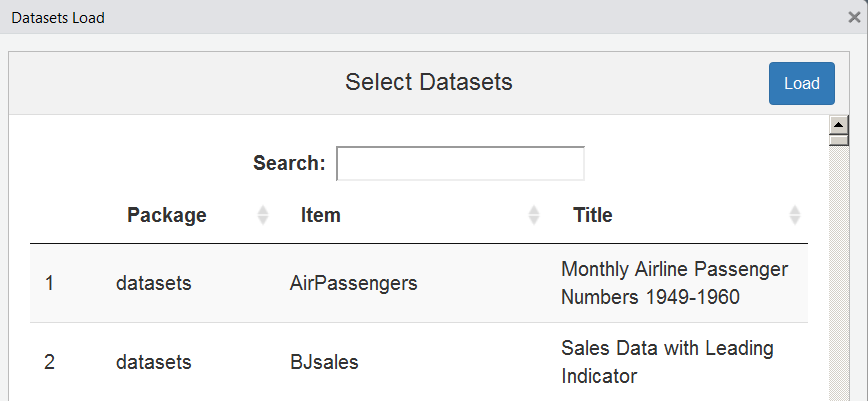
\includegraphics{figure/datasetsload.PNG}

\end{frame}

\begin{frame}{Excursus
\href{https://cran.r-project.org/web/packages/addinslist/README.html}{RStudio
Addins}}
\protect\hypertarget{excursus-rstudio-addins}{}

\begin{itemize}
\tightlist
\item
  In the upper right corner there is a button Addins
\end{itemize}

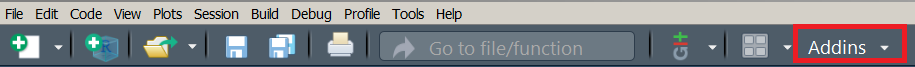
\includegraphics{figure/addins.PNG}

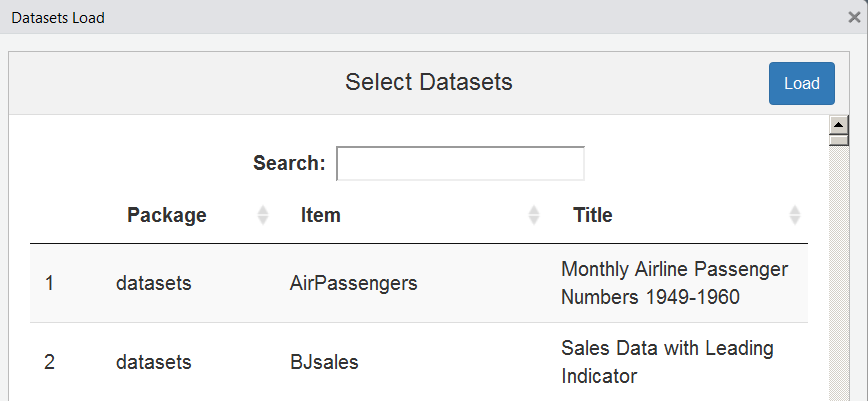
\includegraphics{figure/datasetsload.PNG}

\end{frame}

\begin{frame}[fragile]{Exercise: load built-in data}
\protect\hypertarget{exercise-load-built-in-data}{}

\begin{block}{Load the the built-in dataset \texttt{mtcars}}

\begin{enumerate}
[1)]
\tightlist
\item
  How many observations and variables are available?
\item
  What is the object structure of the variables?
\end{enumerate}

\end{block}

\begin{block}{Interactive data table}

\begin{enumerate}
[1)]
\setcounter{enumi}{2}
\tightlist
\item
  Create an interactive data table
\end{enumerate}

\end{block}

\end{frame}

\begin{frame}[fragile]{\href{https://github.com/lbusett/insert_table}{\textbf{Inserting
data}}}
\protect\hypertarget{inserting-data}{}

\begin{itemize}
\tightlist
\item
  \href{https://github.com/lbusett/insert_table}{\textbf{RStudio addin
  for inserting data}}
\end{itemize}

\begin{Shaded}
\begin{Highlighting}[]
\NormalTok{devtools}\OperatorTok{::}\KeywordTok{install_github}\NormalTok{(}\StringTok{"lbusett/insert_table"}\NormalTok{)}
\end{Highlighting}
\end{Shaded}

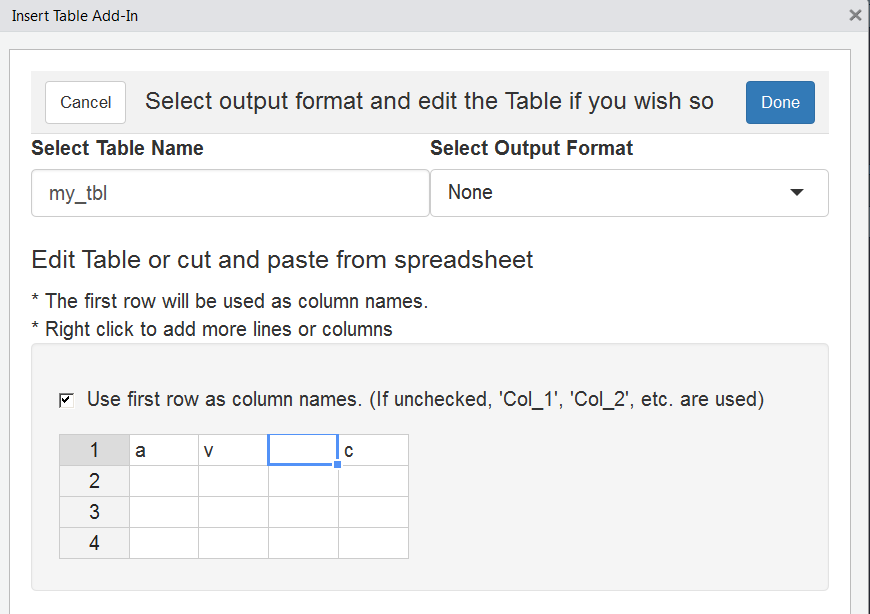
\includegraphics{figure/inserttable.PNG}

\end{frame}

\begin{frame}[fragile]{\href{https://www.r-exercises.com/2018/01/27/Groups-Comparison-With-ANOVA-Solutions/}{The
\texttt{file.choose} option}}
\protect\hypertarget{the-file.choose-option}{}

\begin{itemize}
\tightlist
\item
  You can browse through the directory with \texttt{file.choose}:
\end{itemize}

\begin{Shaded}
\begin{Highlighting}[]
\NormalTok{dat <-}\StringTok{ }\KeywordTok{read.csv}\NormalTok{(}\KeywordTok{file.choose}\NormalTok{())}
\end{Highlighting}
\end{Shaded}

\begin{itemize}
\tightlist
\item
  If you run the command line above a window is opened and you can
  browse in the file system.
\item
  That also works with other import functions
\end{itemize}

\end{frame}

\begin{frame}[fragile]{Creating an example data record}
\protect\hypertarget{creating-an-example-data-record}{}

\begin{Shaded}
\begin{Highlighting}[]
\NormalTok{A <-}\StringTok{ }\KeywordTok{c}\NormalTok{(}\DecValTok{1}\NormalTok{,}\DecValTok{2}\NormalTok{,}\DecValTok{3}\NormalTok{,}\DecValTok{4}\NormalTok{)}
\NormalTok{B <-}\StringTok{ }\KeywordTok{c}\NormalTok{(}\StringTok{"A"}\NormalTok{,}\StringTok{"B"}\NormalTok{,}\StringTok{"C"}\NormalTok{,}\StringTok{"D"}\NormalTok{)}

\NormalTok{mydata <-}\StringTok{ }\KeywordTok{data.frame}\NormalTok{(A,B)}
\end{Highlighting}
\end{Shaded}

\begin{Shaded}
\begin{Highlighting}[]
\NormalTok{mydata}
\end{Highlighting}
\end{Shaded}

\begin{longtable}[]{@{}rl@{}}
\toprule
A & B\tabularnewline
\midrule
\endhead
1 & A\tabularnewline
2 & B\tabularnewline
3 & C\tabularnewline
4 & D\tabularnewline
\bottomrule
\end{longtable}

\end{frame}

\begin{frame}[fragile]{Overview data import/export}
\protect\hypertarget{overview-data-importexport}{}

\begin{itemize}
\tightlist
\item
  if you continue working with R, \texttt{.RData} or
  \href{https://www.fromthebottomoftheheap.net/2012/04/01/saving-and-loading-r-objects/}{\textbf{\texttt{rds}}}
  format is the best choice:
\end{itemize}

\begin{Shaded}
\begin{Highlighting}[]
\KeywordTok{save}\NormalTok{(mydata, }\DataTypeTok{file=}\StringTok{"mydata.RData"}\NormalTok{)}
\KeywordTok{saveRDS}\NormalTok{(mydata, }\StringTok{"mydata.rds"}\NormalTok{)}
\end{Highlighting}
\end{Shaded}

\begin{itemize}
\tightlist
\item
  The data set can be imported with \texttt{load}.
\end{itemize}

\begin{Shaded}
\begin{Highlighting}[]
\KeywordTok{load}\NormalTok{(}\StringTok{"mydata.RData"}\NormalTok{)}
\NormalTok{mydata <-}\StringTok{ }\KeywordTok{readRDS}\NormalTok{(}\StringTok{"mydata.rds"}\NormalTok{)}
\end{Highlighting}
\end{Shaded}

\begin{itemize}
\tightlist
\item
  \texttt{saveRDS()} doesn't save the both the object and its name it
  just saves a representation of the object
\end{itemize}

\end{frame}

\begin{frame}{\href{http://uc-r.github.io/data_wrangling/week-2}{Overview
import functions}}
\protect\hypertarget{overview-import-functions}{}

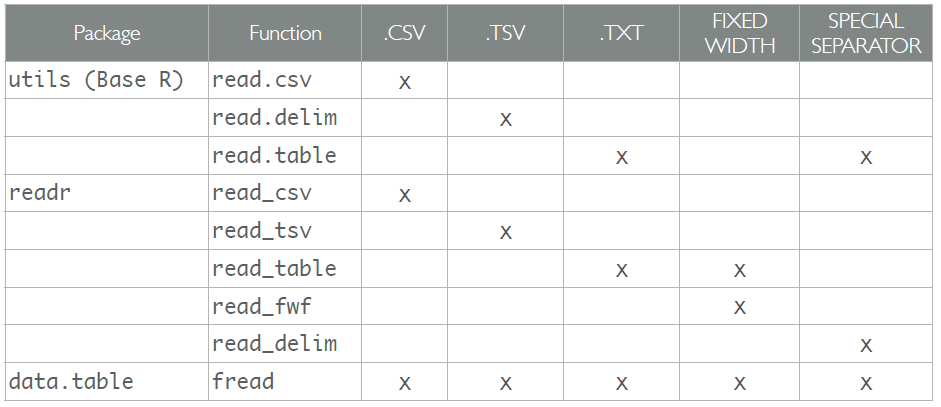
\includegraphics{figure/overviewimportfunctions.PNG}

\end{frame}

\begin{frame}[fragile]{Links and resources}
\protect\hypertarget{links-and-resources}{}

\begin{itemize}
\item
  Introduction to import with R
  (\href{http://is-r.tumblr.com/post/37181850668/reading-writing-stata-dta-files-with-foreign}{\textbf{is.R}})
\item
  \href{https://www.youtube.com/watch?v=WWY8VPh6ryo}{\textbf{Youtube
  video}} on importing data
\item
  Statistical tools for high-throughput data analysis (STHDA) -
  \href{http://www.sthda.com/english/wiki/importing-data-into-r}{\textbf{Importing
  Data Into R}}
\item
  Karlijn Willems -
  \href{https://www.datacamp.com/community/tutorials/r-data-import-tutorial}{\textbf{This
  R Data Import Tutorial Is Everything You Need}}
\item
  \href{https://r4ds.had.co.nz/data-import.html}{\textbf{R for data
  science book}}
\item
  The
  \href{https://cran.r-project.org/web/packages/labelled/labelled.pdf}{\textbf{R-package
  \texttt{labelled}}} to work with labelled data imported from SPSS or
  stata
\item
  \href{https://cran.r-project.org/doc/manuals/r-release/R-data.html}{Overview
  - \textbf{all import functionalities}}
\end{itemize}

\end{frame}

\end{document}
